\setlength{\tabcolsep}{0.03cm}
\begin{figure}[!ht]
% \centering
% \resizebox{0.51\textwidth}{0.23\textheight}{\begin{tabular}{c c}	
{\begin{tabular}{c c}	
	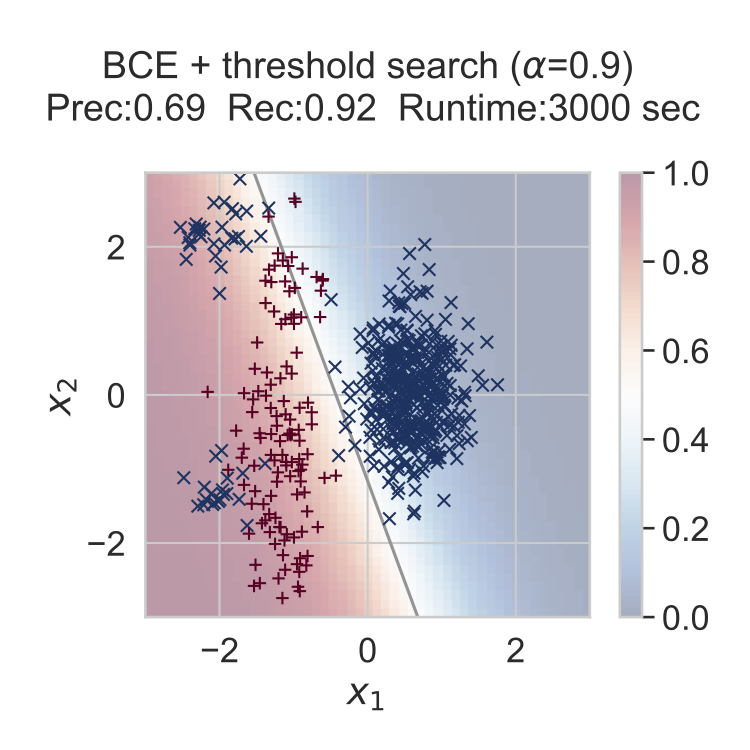
\includegraphics[width=0.49\textwidth,trim={0 .6cm 0 .6cm},clip]{content/chapters/false_alarm_control/figures/BCE_plus_threshold_search_solution_precision_90.jpg}
    &
    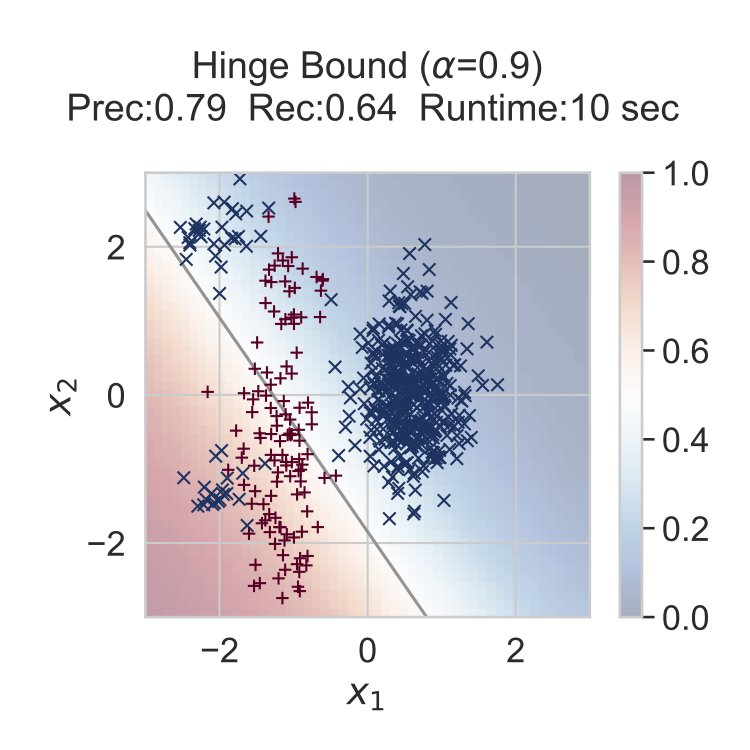
\includegraphics[width=0.49\textwidth,trim={0 .6cm 0 .6cm},clip]{content/chapters/false_alarm_control/figures/hinge_solution_precision_90.jpg}
	\\ 
	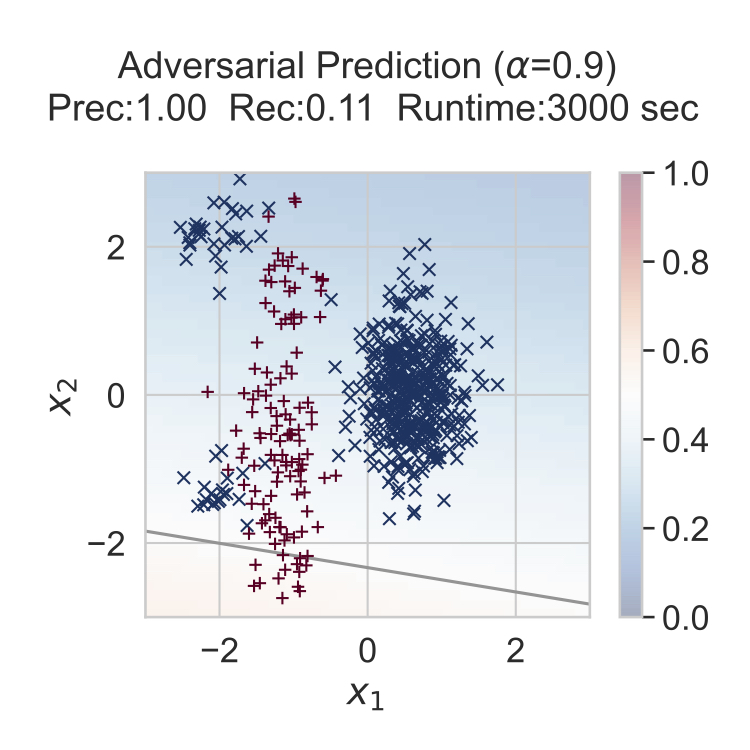
\includegraphics[width=0.49\textwidth,trim={0 .6cm 0 .6cm},clip]{content/chapters/false_alarm_control/figures/adversarial_prediction_precision_90.jpg}
    &
    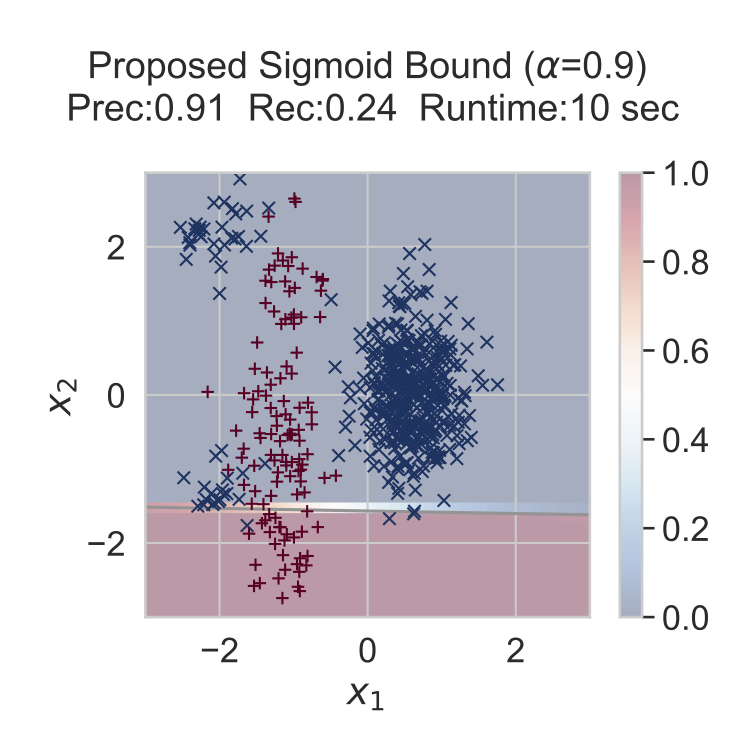
\includegraphics[width=0.49\textwidth,trim={0 .6cm 0 .6cm},clip]{content/chapters/false_alarm_control/figures/sigmoid_solution_precision_90.jpg}
\end{tabular}}
\vspace{-5mm}
\caption[Comparison of decision boundaries from BCE, hinge, adversarial prediction and our sigmoid bounds]{Linear decision boundaries (black lines) found by various methods on toy data when stated goal is to maximizes recall subject to a minimum precision of $\alpha = 0.9$.
Subtitles report precision, recall, and total runtime for each method's solution. 
Red and blue markers represent positive and negative examples, respectively, for the toy dataset used for training (Sec. \ref{sec:synth}).
\emph{Top Left}: Even with post-hoc search, binary cross entropy (BCE) cannot exceed a precision of 0.684. 
\emph{Top Right}: Despite including the desired $\alpha = 0.9$ precision constraint in its objective, \citet{ebanScalableLearningNonDecomposable2017}'s hinge bound cannot satisfy the constraint.
\emph{Bottom}: Both \citet{fathonyAPperfIncorporatingGeneric2020}'s AP method and our proposed sigmoid bound satisfy the precision constraint; ours delivers 2x the recall of the AP solution in $1/300^{th}$ of the time.
}%endcaption
\label{fig:toy_data_precision_90}
\end{figure}